\section{Resultater fra Affinity diagram}
\label{ParametreDatabehandlingAffinityDiagram}
%
%OBS: SKRIV LIGE AT VI BRUGER VAS BI- OG UNIPOLAR, HUSK AT SKRIV HVORDAN DE BYGGES OP
%TJEK OP PÅ AT FORMULERINGERNE ER ENS MED DET DER STÅR PÅ POST ITS
%
Da formålet med projektet er, at udlede hvilke parametre danske rejsende tilskriver interaktionen med en social robot for efterfølgende at udvikle skalaer, som kan bruges til evaluere oplevelsen af interaktionen med robotten, bør der fremsættes nogle krav for hvordan parametrene udvælges for dernæst at formulere dem til skalaer. 

For at udlede parametrene fokuseres der på én grøn kategori af gangen, hvorfra parametrene formuleres på baggrund af både pink og blå labels. Parametrene vil formuleres som et udsagn, der kan evalueres på en skala, hvorfor parametre noteres med et \textit{S} på en orange \textit{sticky note}. De orange \textit{sticky notes} kan derudover indeholde design idéer \textit{DI}, indsigter \textit{I} samt idéer til det efterfølgende testdesign \textit{TD}. Der er i alt dannet 50 orange \textit{sticky notes}, hvoraf 42 er formuleret som potentielle udsagn, der kan evalueres på en skala, seks design idéer, én indsigt og ét foreslag til testdesign. 

Først vil hver af de 10 grønne kategorier blive præsenteret sammen med tilhørende potentielle udsagn. Derefter vil der fokuseres på dannelsen af de endelige skalaer.
%
\subsection*{Interagerer ikke med R}
%
\begin{figure}[H]
\centering
\includegraphics[width = 0.7\textwidth, angle = -90]{Figure/AffinityDiagram/InteragererIkkeMedR} 
\caption{Oversigt over den grønne kategori: \textit{Interagerer ikke med R}, hvor er \textit{R} angiver robot, med tilhørende \textit{affinity notes} placeret under henholdvist blå og pink labels, samt de udarbejde orange \textit{sticky notes}.}
\label{fig:AFInteragererIkkeMedR}
\end{figure}
\noindent
%
På \autoref{fig:AFInteragererIkkeMedR} fremgår to orange \textit{sticky notes}, hvoraf én er en idé til det næste testdesign, som relaterer sig til at de rejsende, der interagerer med robotten men ikke ender med at følge efter robotten stoppes og spørges ind til hvorfor de stoppede interaktionen. Den anden orange \textit{sticky note} er et potentielt skala spørgsmål:\blankline 
%
\begin{enumerate}
  \item Er det let at undgå R/Er det let at ignorer R\blankline
\end{enumerate} 
\noindent
%
Til ovenstående potentielle skala spørgsmål kan følgende labels anvendes:
%
\begin{table}[H]
	\centering
	\begin{tabular}{l|c|c|c}
		SQ     & Venstre label & Midt punkt & Højre label \\\hline
		1   & Slet ikke & - & Ekstremt meget                 
	\end{tabular}
\caption{Skala labels vedrørende hvor let det er at undgå robotten.}
	\label{tab:IgnorerR} 
\end{table}
\noindent
%
Baseret på det potentielle skala spørgsmål samt tilhørende labels, der fremgår i \autoref{tab:IgnorerR}, vil det udgøre en unipolar skala uden et midt punkt. 
%MÅSKE IKKE DE BEDSTE LABELS I FORHOLD TIL SPØRGSMÅLET?
%
\subsection*{Skærmen virker ikke}
%
\begin{figure}[H]
\centering
\includegraphics[width = 0.9\textwidth]{Figure/AffinityDiagram/SkaermenVirkerIkke} 
\caption{Oversigt over den grønne kategori: \textit{Skærmen virker ikke} med tilhørende \textit{affinity notes} placeret under henholdvist blå og pink labels, samt de udarbejde orange \textit{sticky notes}.}
\label{fig:AFSkaermVirkerIkke}
\end{figure}
\noindent
%
Da de to orange \textit{sticky notes} vedrører den samme problemstilling, at skærmen forvoldte problemer vælges det er sætte de to sammen og omformulere dem til følgende:\blankline
%
\begin{enumerate}
  \item Hvordan synes du skærmen virkede\blankline
\end{enumerate}
%
Til ovenstående potentielle skala spørgsmål kan følgende labels anvendes:
%
\begin{table}[H]
	\centering 
	\begin{tabular}{l|c|c|c}
		SQ     & Venstre label & Midt punkt & Højre label \\\hline
		1   & Ekstremt dårligt & Intet label & Ekstremt godt                 
	\end{tabular}
\caption{Skala labels vedrørende skærmen på robotten.}
	\label{tab:SkaermenR}
\end{table}
\noindent
%
Det potentielle skala spørgsmål vil blive evalueret på en bipolar skala med et unavngivet midt punkt.
%
\subsection{R kan assistere mennesker}
%
\begin{figure}[H]
\centering
\includegraphics[width = 0.9\textwidth]{Figure/AffinityDiagram/RKanAssistereMennesker} 
\caption{Oversigt over den grønne kategori: \textit{R kan assistere mennesker}, hvor \textit{R} angiver robot og \textit{L} angiver lufthavn, med tilhørende \textit{affinity notes} placeret under henholdvist blå og pink labels, samt de udarbejde orange \textit{sticky notes}.}
\label{fig:AFRKanAssistereMennesker}
\end{figure}
\noindent
%
Baseret på de fire potentielle skala spørgsmål vælges det at sammensætte: \textit{Jeg kan bruge R til at finde rundt i L} og \textit{Jeg føler at R kan hjælpe mig} til et samlet potentielt skala spørgsmål, som fremgår i nedenstående. Derudover er fremgår der en design idé på \autoref{fig:AFRKanAssistereMennesker}, som vedrører at robotten bør kunne hjælpe på forskellige sprog og ikke kun på dansk.\blankline 
%
\begin{enumerate}
  \item Jeg oplever at R's hjælp som personlig
  \item Jeg føler at R kan hjælpe mig
  \item R kan hjælpe mig så jeg ikke behøver at spørge personale\blankline
\end{enumerate}
\noindent
%
Til hver af de tre ovenstående potentielle skala spørgsmål kan følgende labels anvendes:
%
\begin{table}[H]
	\centering
	\begin{tabular}{l|c|c|c}
		SQ     & Venstre label & Midt punkt & Højre label \\\hline
		1   & Slet ikke personlig & - & Ekstremt personlig          \\\hline
		2   & Helt uenig & Intet label & Helt enig   \\\hline
		3   & Helt uenig & Neutral & Helt enig  \\\hline
	\end{tabular}
\caption{Skala labels vedrørende hvorvidt robotten kan assistere mennesker.}
	\label{tab:AssistererMennesker}
\end{table}
\noindent
%
Skalaen vedrørende hvorvidt robottens hjælp opleves som værende personlig vil blive evalueret på en unipolar skala. Hvor de to andre potentielle skala spørgsmål begge vil blive evalueret på en bipolar skala med et midt punkt henholdvist unavngivet og angivet med \textit{Neutral}.
\newpage
%
\subsection*{R's væremåde}
%
\begin{figure}[H]
\centering
\includegraphics[width = 0.9\textwidth]{Figure/AffinityDiagram/RsVaeremaade} 
\caption{Oversigt over den grønne kategori: \textit{R's væresmåde}, hvor \textit{R} angiver robot, med tilhørende \textit{affinity notes} placeret under henholdvist blå og pink labels, samt de udarbejde orange \textit{sticky notes}.}
\label{fig:AFRsVaeremaade}
\end{figure}
\noindent
%
Ud af de ni orange \textit{sticky notes} er to design idéer hvor én relatere sig til at det bør overvejes om robotten skal tale og den anden relatere sig til at robotten skal tilpasse sine bevægelser afhængigt af brugerens bevægelser. Derudover er det valgt at sammensætte \textit{Jeg synes R's bevægelser er behagelige} og \textit{Jeg synes R har rolige bevægelser} til ét potentielt skala spørgsmål, listet som det første i nedenstående. Ydermere er det valgt at sammensætte \textit{Jeg oplevede R's hastighed som værende hurtig/langsom} og \textit{Jeg synes at R's hastighed er for langsom/for hurtig} til ét potentiel skala spørgsmål der vedrører robottens hastighed, listet som nummer to i nedenstående. De tre resterende bibeholdes: \blankline 
%
\begin{enumerate}
  \item Jeg synes R's bevægelser er... 
  \item Jeg synes at R's hastighed er... 
  \item Jeg synes R er irriterende...
  \item Jeg synes R er levende...
  \item Jeg synes R er anmassende...\blankline
\end{enumerate}
%
Til hver af de fem ovenstående potentielle skala spørgsmål kan følgende labels anvendes:
%
\begin{table}[H]
	\centering 
	\begin{tabular}{l|c|c|c}
		SQ     & Venstre label & Midt punkt & Højre label \\\hline
		1   & For rolige & Intet label & For vilde     \\\hline
		2   & For langsom & Fin & For hurtig   \\\hline
		3   & Slet ikke irriterende & - & Ekstremt irriterende \\\hline
	 	4   & Slet ikke levende & - & Ekstremt levende         \\\hline
		5   & Slet ikke anmassende & - & Ekstremt anmassende             
	\end{tabular}
	\caption{Skala labels vedrørende robottens væremåde.}
	\label{tab:VaeremaadeSkala}
\end{table}
\noindent
%
De to første potentielle skala spørgsmål vil begge blive evalueret på en bipolar skala med et midt punkt henholdvist uden et label og med label: \textit{Fin}. De tre resterende vil hver blive evalueret på en unipolar skala.
%
\subsection*{Henvendelse}
%
\begin{figure}[H]
\centering
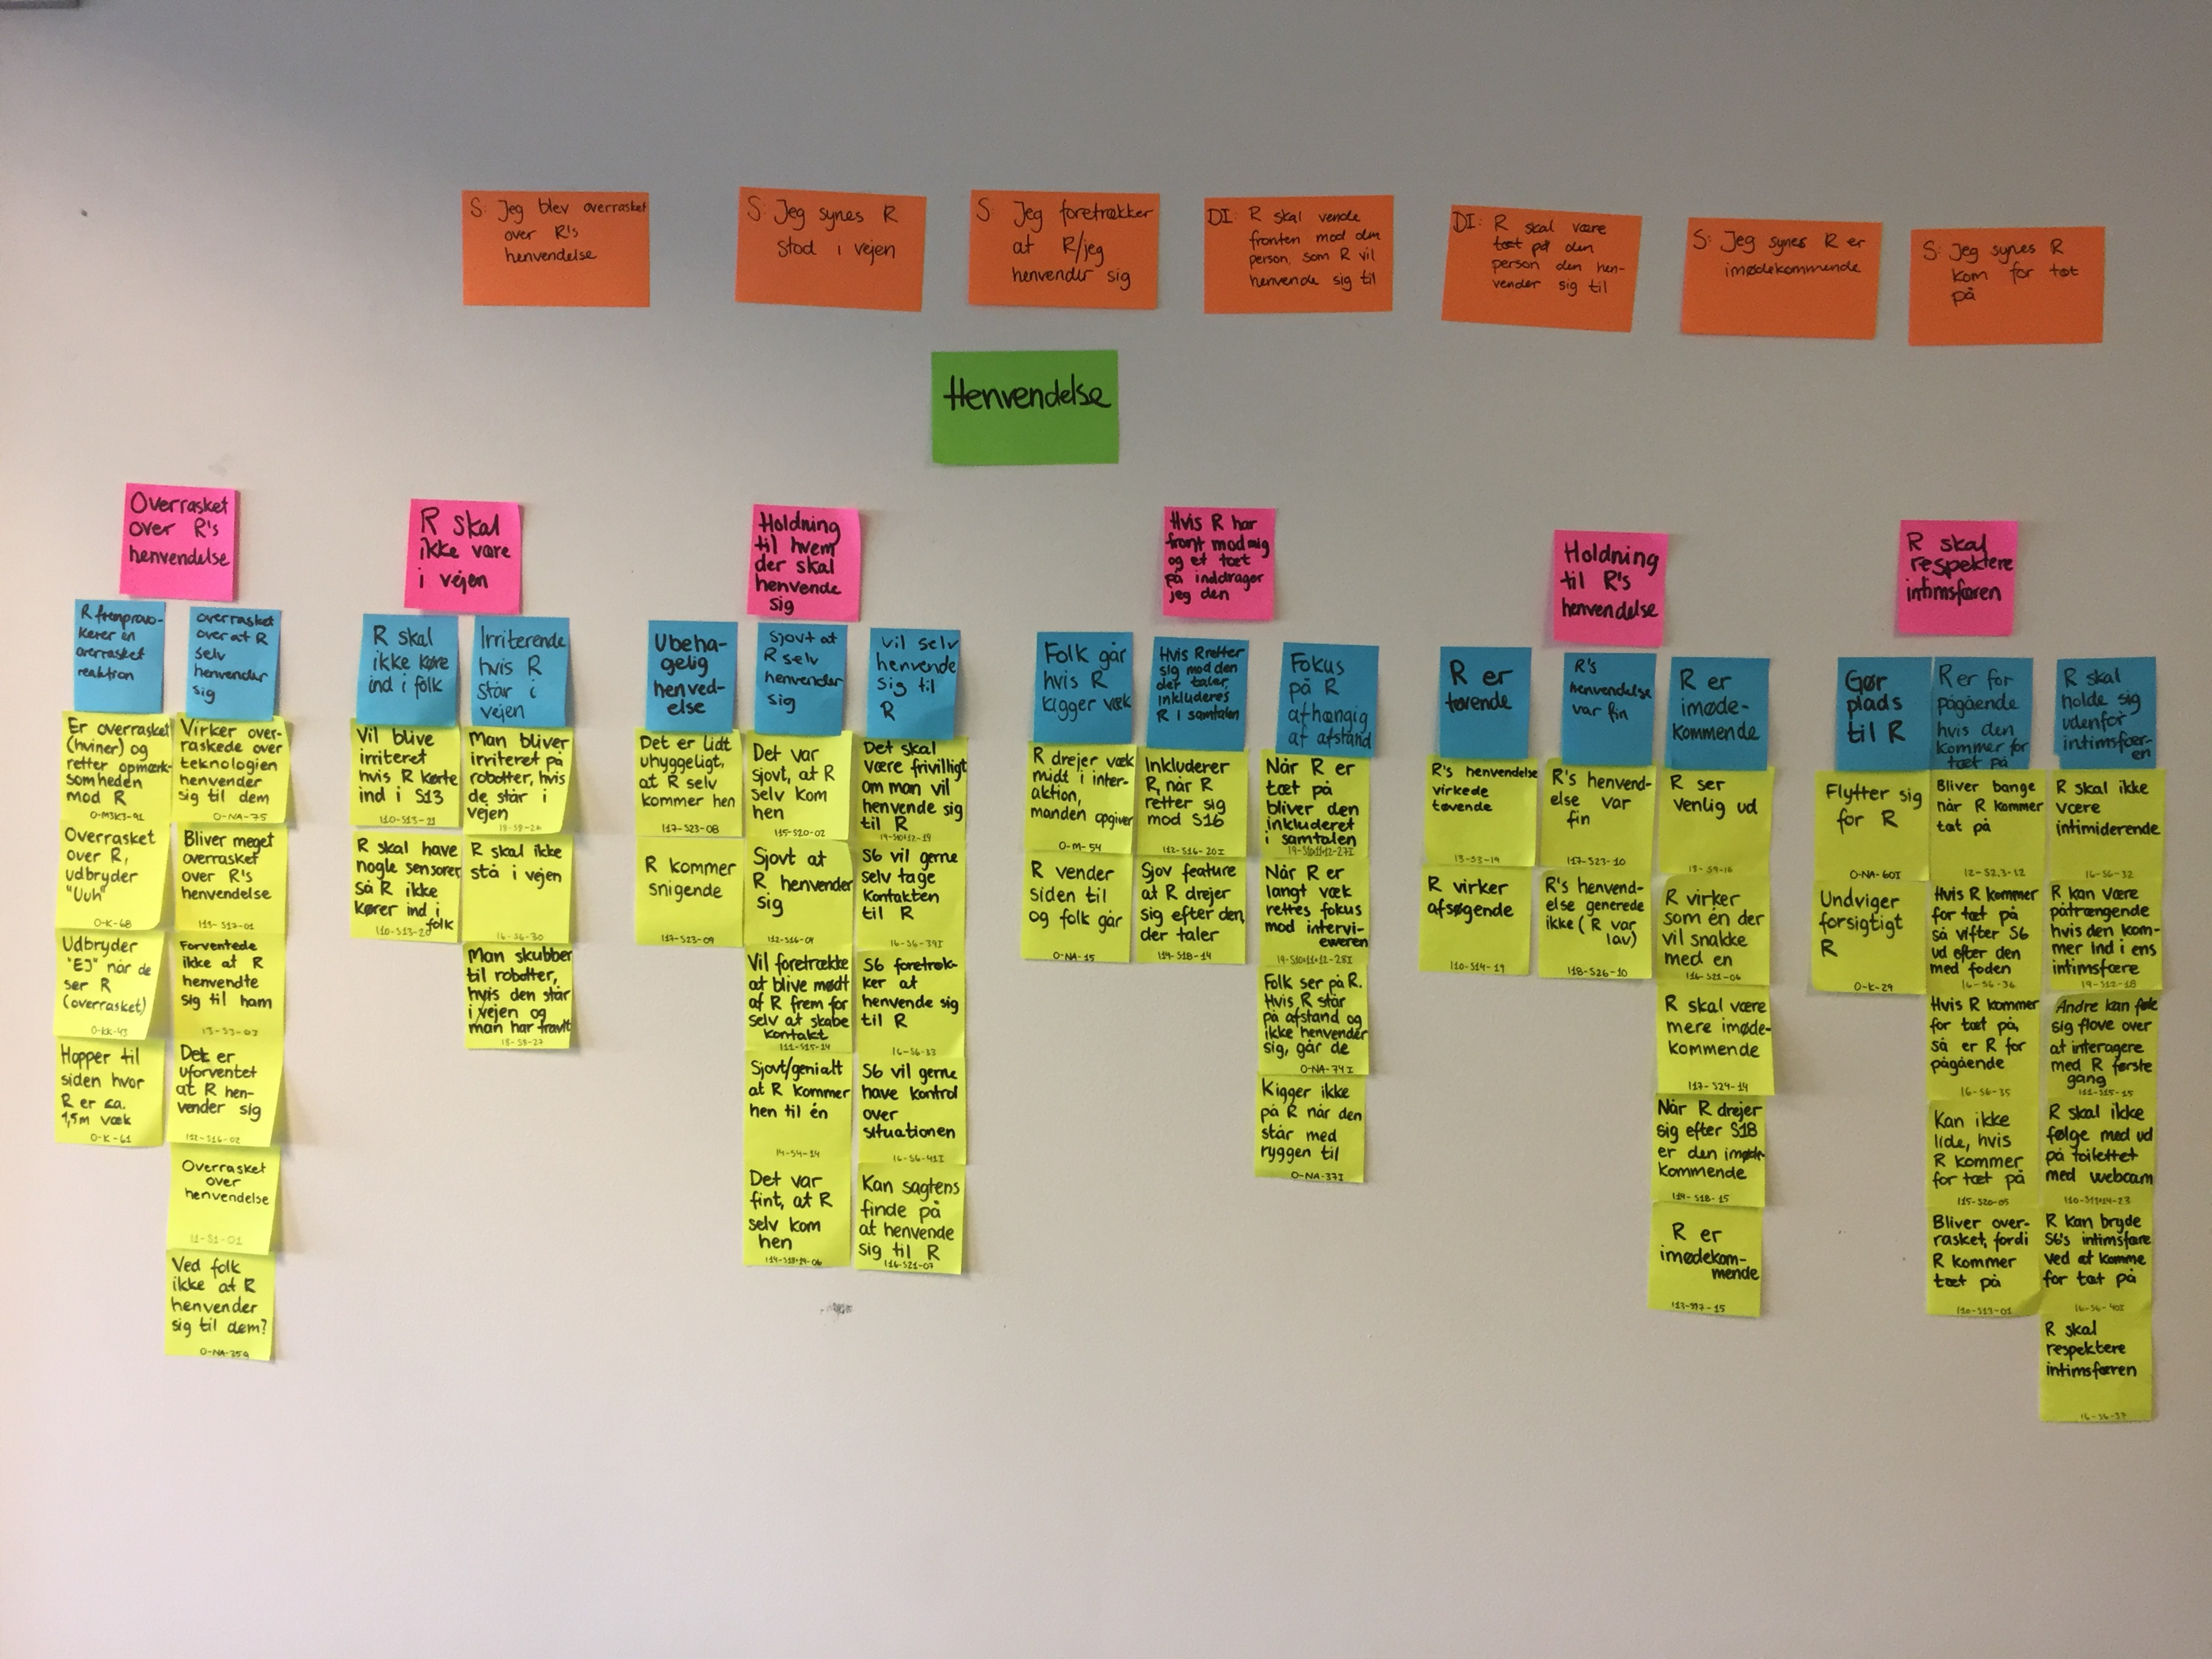
\includegraphics[width = 0.9\textwidth]{Figure/AffinityDiagram/Henvendelse} 
\caption{Oversigt over den grønne kategori: \textit{Henvendelse} med tilhørende \textit{affinity notes} placeret under henholdvist blå og pink labels, samt de udarbejde orange \textit{sticky notes}.}
\label{fig:AFHenvendelse}
\end{figure}
\noindent
%
To ud af de syv orange \textit{sticky notes} er angivet som design idéer vedrørende robottens position relativt til brugeren, hvor robotten fortrinvist skal vende fronten mod brugeren samt være tæt på personen. Det vælges at ekskludere \textit{Jeg foretrækker at R/jeg henvender sig}, da det ikke er en parameter, der for en designer er mulig at ændre på. Derudover vælges det at omformulere \textit{Jeg synes R kom for tæt på} til \textit{Jeg synes R er intimiderende}. Denne omformulering er baseret på dels de blå labels samt \textit{affinity notes} kategoriseret under den pink label: \textit{R skal respektere intimsfæren}. Dette medføre at følgende potentielle skala spørgsmål formuleres: \blankline
%
\begin{enumerate}
  \item Jeg synes R er imødekommende
  \item Jeg synes R kom for tæt på
  \item Jeg synes R stod i vejen
  \item Jeg blev overrasket over R's henvendelse 
  \item Jeg synes R er intimiderende\blankline
\end{enumerate}
%
Til hver af de fem ovenstående potentielle skala spørgsmål kan følgende labels anvendes:
%
\begin{table}[H]
	\centering
	\begin{tabular}{l|c|c|c}
		SQ     & Venstre label & Midt punkt & Højre label \\\hline
		1   & Meget afvisende & Intet label & Meget imødekommende         \\\hline
		2   & For langt væk & Tilpas & For tæt på    \\\hline
		3   & Slet ikke i vejen & -  & Ekstremt i vejen  \\\hline
	 	4   & Slet ikke overrasket &  -  & Ekstremt overrasket \\\hline
		5   & Slet ikke intimiderende & - & Ekstremt intimiderende           
	\end{tabular}
	\caption{Skala labels vedrørende robottens henvendelse.}
	\label{tab:HenvendelseSkala} 
\end{table}
\noindent
%
Baseret på \autoref{tab:HenvendelseSkala} vil de to første potentielle skala spørgsmål blive evalueret på en bipolar skala med et midt punk som henholdvist er unavngivet og navngivet med \textit{Tilpas}. De tre resterende potentielle skala spørgsmål vil hver blive evalueret på en unipolar skala.
\newpage
%
\subsection*{R's udseende}
%
\begin{figure}[H]
\centering
\includegraphics[width = 0.9\textwidth]{Figure/AffinityDiagram/RsUdseende} 
\caption{Oversigt over den grønne kategori: \textit{R's udseende}, hvor \textit{R} angiver robot, med tilhørende \textit{affinity notes} placeret under henholdvist blå og pink labels, samt de udarbejde orange \textit{sticky notes}.}
\label{fig:AFRsUdseende}
\end{figure}
\noindent
%
På \autoref{fig:AFRsUdseende} fremgår der én design idé, som vedrører at robotten automatisk skal indstille sin højde afhængigt af brugerens højde. Det vælges at sammensætte \textit{Jeg oplevede R's højde som værende meget høj/meget lav} og \textit{Jeg synes at R's højde er for høj/for lav} til et enkelt potentielt skala spørgsmål vedrørende robottens højde. Da det ikke er muligt for en designer at påvirke hvad en potentiel bruger foretrækker vælges det at sammensætte \textit{Jeg foretrækker at R ser menneskelig ud} og \textit{Jeg synes at R ser menneskelig ud}. De potentielle skala spørgsmål er som følger: \blankline
% 
\begin{enumerate}
  \item Jeg synes at R's højde er... 
  \item Jeg synes R er elegant...
  \item Jeg synes R ser menneskelig ud... 
  \item Jeg kan godt lide R's udseende...\blankline
\end{enumerate}
%
Til hver af de fem ovenstående potentielle skala spørgsmål kan følgende labels anvendes:\blankline
%
\begin{table}[H]
	\centering
	\begin{tabular}{l|c|c|c}
		SQ     & Venstre & Midt punkt & Højre label \\\hline
		1   & For lav  & Fin & For høj        \\\hline
		2   & Slet ikke elegant & - & Ekstremt elegant         \\\hline
		3   & Slet ikke menneskelig & - & Ekstremt menneskelig         \\\hline
	 	4   & Helt uenig & - & Helt enig         \\\hline
		5   & Slet ikke forskrækket & -  & Ekstremt forskrækket           
	\end{tabular}  
	\caption{Skala labels vedrørende robottens udseende.}
	\label{tab:UdseendeSkala}       
\end{table}
\noindent
%
\newpage
%
\subsection*{Interesse for R}
%
\begin{figure}[H]
\centering
\includegraphics[width = 0.9\textwidth]{Figure/AffinityDiagram/InteresseForR} 
\caption{Oversigt over den grønne kategori: \textit{Interesse for R}, hvor \textit{R} angiver robot, med tilhørende \textit{affinity notes} placeret under henholdvist blå og pink labels, samt de udarbejde orange \textit{sticky notes}.}
\label{fig:AFInteresseForR}
\end{figure}
\noindent
%
\begin{enumerate}
  \item R fangede min opmærksomhed
  \item Jeg synes at R er spændende
\end{enumerate}
%
\begin{table}[H]
	\centering 
	\begin{tabular}{l|c|c|c}
		SQ     & Venstre label & Midt punkt & Højre label \\\hline
		1   & Slet ikke & - & Ekstremt meget          \\\hline
		2   & Slet ikke spændende & - & Ekstremt spændende                 
	\end{tabular}
\caption{Skala labels vedrørende interesse for robotten.}
	\label{tab:InteresseForR}
\end{table}
\noindent
%
\newpage
%
\subsection*{Positiv overfor R}
%
\begin{figure}[H]
\centering
\includegraphics[width = 0.9\textwidth]{Figure/AffinityDiagram/PositivOverforR} 
\caption{Oversigt over den grønne kategori: \textit{Positiv overfor R}, hvor \textit{R} angiver robot, med tilhørende \textit{affinity notes} placeret under henholdvist blå og pink labels, samt de udarbejde orange \textit{sticky notes}.}
\label{fig:AFPositivOverforR}
\end{figure}
\noindent
%
%
\begin{enumerate}
  \item Jeg synes R er sød
  \item Jeg synes R er sjov
  \item Jeg synes R er sej
  \item Jeg kan godt lide at blive betjent af R
\end{enumerate}
%
\begin{table}[H]
	\centering
	\begin{tabular}{l|c|c|c}
		SQ     & Venstre label & Midt punkt & Højre label \\\hline
		1   & Slet ikke sød & - & Ekstremt sød      \\\hline
		2   & Slet ikke sjov & - & Ekstremt sjov \\\hline
		3   & Slet ikke sej & - & Ekstremt sej \\\hline
		4   & Slet ikke & - & Ekstremt meget
	\end{tabular}
\caption{Skala labels vedrørende ens positive indstilling i henhold til robotten.}
\label{tab:PositivR} 
\end{table}
\noindent
%
\newpage
%
\subsection{Kendskab til teknologi}
%
\begin{figure}[H]
\centering
\includegraphics[width = 0.9\textwidth]{Figure/AffinityDiagram/KendskabTilTeknologi} 
\caption{Oversigt over den grønne kategori: \textit{Kendskab til teknologi} med tilhørende \textit{affinity notes} placeret under henholdvist blå og pink labels, samt de udarbejde orange \textit{sticky notes}.}
\label{fig:AFKendskabTilTeknologi}
\end{figure}
\noindent
%
%
\begin{enumerate}
  \item Hvordan var det at bruge R (Jeg synes at R er nem at bruge (kommer fra positiv overfor R) og Jeg har brug for hjælp til at bruge R)
  \item Hvor meget kenderskab har du til teknologi/robotter (Jeg synes at R minder om noget jeg kender, Jeg har erfaring med robotter og Min erfaring med teknologi har betydning for min oplevelse af R)
\end{enumerate}
%
Skala spørgsmål 2 vil blive brugt i forbindelse med demografi.
%
\begin{table}[H]
	\centering 
	\begin{tabular}{l|c|c|c}
		SQ     & Venstre label & Midt punkt & Højre label \\\hline
		1   & Ekstremt svært & Intet label & Ekstremt nemt          \\\hline
		2   & Slet ingen kendskab & - & Ekstremt meget kendskab 
	\end{tabular}
\caption{Skala labels vedrørende kendskab til teknologi.}
	\label{tab:KendskabTilTek}
\end{table}
\noindent
%
\newpage
%
\subsection*{Tillid til R}
%
\begin{figure}[H]
\centering
\includegraphics[width = 0.9\textwidth]{Figure/AffinityDiagram/TillidTilR} 
\caption{Oversigt over den grønne kategori: \textit{Tillid til R}, hvor \textit{R} angiver robot, med tilhørende \textit{affinity notes} placeret under henholdvist blå og pink labels, samt de udarbejde orange \textit{sticky notes}.}
\label{fig:AFTillidTilR}
\end{figure}
\noindent
%
\begin{enumerate}
  \item Jeg føler mig tryg ved R
  \item Jeg regner med at R følger mig hen til det sted jeg har valgt
  \item R gjorde mig forskrækket\blankline
\end{enumerate}
%
\begin{table}[H]
	\centering 
	\begin{tabular}{l|c|c|c}
		SQ  & Venstre label & Midt punkt & Højre label \\\hline
		1   & Ekstremt utryg & Intet label & Ekstremt tryg  \\\hline
		2   & Helt uenig & Neutral & Helt enig 
	\end{tabular} 
	\caption{Skala labels vedrørende tillid til robotten.}
	\label{tab:TillidSkala}       
\end{table}
\noindent
%
\newpage
%